%=================================================================
% CSE 4345 — Big Data Analytics
% Week 3, Part 2: Seminal Research & Case Study
% Department of CSE, Premier University
%
% SEMINAL PAPER:
%   Ghemawat, Gobioff & Leung (2003) — The Google File System
%   SOSP 2003 (cited >14,000 times)
%
% CASE STUDY:
%   Yahoo! Hadoop Cluster (2006–2011) — First Industrial-Scale
%   Open-Source Distributed File System Deployment
%=================================================================

\documentclass[aspectratio=169,10pt]{beamer}

%---------- Packages ----------
\usepackage[utf8]{inputenc}
\usepackage[T1]{fontenc}
\usepackage{booktabs}
\usepackage{xcolor}
\usepackage{tikz}
\usetikzlibrary{shapes.geometric, positioning, arrows.meta, decorations.pathreplacing}
\usepackage{amsmath}
\usepackage{graphicx}
\usepackage{multicol}
\usepackage{enumerate}
\usepackage{array}

%---------- Theme ----------
\usetheme{Madrid}

%---------- Premier University Color Identity ----------
\definecolor{PUNavy}{RGB}{10,36,99}
\definecolor{PUGold}{RGB}{197,151,37}
\definecolor{PULightBlue}{RGB}{210,228,255}
\definecolor{PUTeal}{RGB}{0,100,100}
\definecolor{PUGray}{RGB}{90,90,90}
\definecolor{PURed}{RGB}{160,30,30}
\definecolor{PUGreen}{RGB}{30,120,60}
\definecolor{PUPurple}{RGB}{90,30,120}
\definecolor{PUOrange}{RGB}{190,90,20}

\setbeamercolor{palette primary}{bg=PUNavy, fg=white}
\setbeamercolor{palette secondary}{bg=PUNavy!85, fg=white}
\setbeamercolor{palette tertiary}{bg=PUNavy!70, fg=white}
\setbeamercolor{palette quaternary}{bg=PUNavy, fg=white}
\setbeamercolor{structure}{fg=PUNavy}
\setbeamercolor{title}{bg=PUNavy, fg=PUGold}
\setbeamercolor{subtitle}{fg=white}
\setbeamercolor{frametitle}{bg=PUNavy, fg=PUGold}
\setbeamercolor{alerted text}{fg=PUGold!85!black}
\setbeamercolor{block title}{bg=PUNavy, fg=white}
\setbeamercolor{block body}{bg=PULightBlue!45}
\setbeamercolor{block title alerted}{bg=PUGold!80!black, fg=white}
\setbeamercolor{block body alerted}{bg=PUGold!12}
\setbeamercolor{block title example}{bg=PUTeal, fg=white}
\setbeamercolor{block body example}{bg=PUTeal!10}
\setbeamercolor{section in toc}{fg=PUNavy}
\setbeamercolor{itemize item}{fg=PUGold!80!black}
\setbeamercolor{itemize subitem}{fg=PUNavy!70}

\setbeamertemplate{navigation symbols}{}
\setbeamertemplate{itemize item}{\scriptsize\raise1.5pt\hbox{\textbullet}}
\setbeamertemplate{itemize subitem}{\scriptsize\raise1pt\hbox{--}}

%---------- Section separator ----------
\AtBeginSection[]{
  \begin{frame}[plain]
    \vfill
    \centering
    \begin{beamercolorbox}[sep=12pt,center,shadow=true,rounded=true]{block title}
      \usebeamerfont{title}\insertsectionhead\par
    \end{beamercolorbox}
    \vfill
  \end{frame}
}

%---------- Helper: citation box ----------
\newenvironment{paperbox}[1]{%
  \setbeamercolor{block title}{bg=PUNavy!90,fg=PUGold}
  \setbeamercolor{block body}{bg=PUNavy!6}
  \begin{block}{#1}}{%
  \end{block}}

%---------- Custom footline ----------
\setbeamertemplate{footline}{
  \leavevmode\hbox{%
    \begin{beamercolorbox}[wd=.333\paperwidth,ht=2.25ex,dp=1ex,center]{palette primary}
      \usebeamerfont{author in head/foot}\insertshortauthor
    \end{beamercolorbox}%
    \begin{beamercolorbox}[wd=.334\paperwidth,ht=2.25ex,dp=1ex,center]{palette secondary}
      \usebeamerfont{title in head/foot}\insertshorttitle
    \end{beamercolorbox}%
    \begin{beamercolorbox}[wd=.333\paperwidth,ht=2.25ex,dp=1ex,right]{palette primary}
      \usebeamerfont{date in head/foot}
      \insertframenumber{} / \inserttotalframenumber\hspace*{2ex}
    \end{beamercolorbox}}%
  \vskip0pt%
}

%---------- Title metadata ----------
\title[CSE 4345 \textbar{} Week 3, Part 2]{CSE 4345: Big Data Analytics}
\subtitle{Week 3, Part 2 \textemdash\ Seminal Research \& Case Study}
\author[Dept.\ of CSE]{Department of Computer Science \& Engineering\\[4pt]
       \small Premier University, Chittagong}
\institute{}
\date{Semester 2026}

%=================================================================
\begin{document}
%=================================================================

%----------------------------------------------------------------
% TITLE SLIDE
%----------------------------------------------------------------
\begin{frame}
  \titlepage
\end{frame}

%----------------------------------------------------------------
% PART 2 OVERVIEW
%----------------------------------------------------------------
\begin{frame}{Part 2 Overview — Week 3}
  \begin{columns}[T]
    \column{0.47\textwidth}
      \begin{block}{Today's Agenda}
        \tableofcontents
      \end{block}

    \column{0.50\textwidth}
      \begin{exampleblock}{Seminal Paper Covered}
        \begin{enumerate}
          \item Ghemawat, S., Gobioff, H., \& Leung, S.-T. (2003).
                \textit{The Google File System.}
                ACM SOSP 2003. Bolton Landing, NY.
        \end{enumerate}
      \end{exampleblock}
      \vspace{6pt}
      \begin{alertblock}{Case Study}
        Yahoo!\ Hadoop Cluster (2006--2011) — the first industrial-scale
        open-source distributed filesystem deployment,
        scaling from 1{,}000 to 42{,}000 nodes in five years.
      \end{alertblock}
      \vspace{4pt}
      \begin{block}{CLO Addressed}
        \textbf{CLO1} — Understand distributed storage architecture\\
        \textbf{PLO(a,b)}
      \end{block}
  \end{columns}
\end{frame}

%================================================================
\section{Research Paper — Ghemawat, Gobioff \& Leung (2003)}
%================================================================

%----------------------------------------------------------------
\begin{frame}{Research Landscape: Distributed File Systems Timeline}
  \begin{center}
  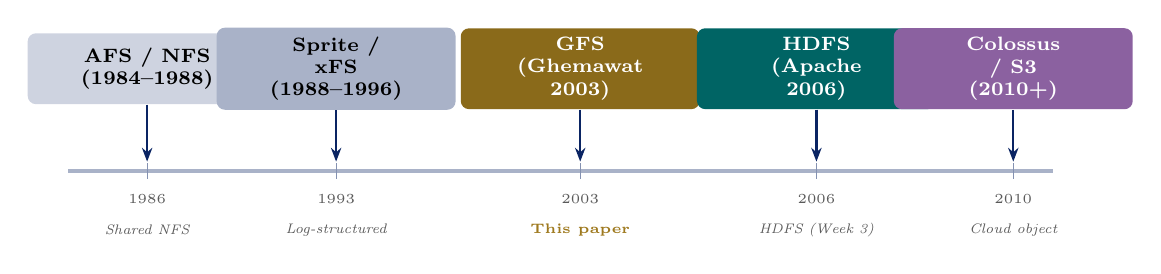
\begin{tikzpicture}[
      nbox/.style={rectangle, rounded corners=3pt, minimum width=3.0cm,
                   minimum height=0.9cm, text width=2.8cm, align=center,
                   font=\scriptsize\bfseries},
      arr/.style={-{Stealth[length=5pt]}, draw=PUNavy, thick}
    ]
    \draw[PUNavy!35, very thick] (0,0) -- (12.5,0);

    \node[nbox, fill=PUNavy!20]              (afs)  at (1.0, 1.3)
          {AFS / NFS\\(1984--1988)};
    \node[nbox, fill=PUNavy!35]              (sprite) at (3.4, 1.3)
          {Sprite /\\xFS\\(1988--1996)};
    \node[nbox, fill=PUGold!70!black, text=white] (gfs) at (6.5, 1.3)
          {GFS\\(Ghemawat\\2003)};
    \node[nbox, fill=PUTeal, text=white]     (hdfs) at (9.5, 1.3)
          {HDFS\\(Apache\\2006)};
    \node[nbox, fill=PUPurple!70, text=white](colo) at (12.0,1.3)
          {Colossus\\/ S3\\(2010+)};

    \foreach \x/\y in {1.0/1986, 3.4/1993, 6.5/2003, 9.5/2006, 12.0/2010}{
      \draw[PUNavy!50] (\x,0.1) -- (\x,-0.1);
      \node[font=\tiny, text=PUGray] at (\x,-0.35) {\y};
    }

    \draw[arr] (afs)   -- (1.0,  0.12);
    \draw[arr] (sprite)-- (3.4,  0.12);
    \draw[arr] (gfs)   -- (6.5,  0.12);
    \draw[arr] (hdfs)  -- (9.5,  0.12);
    \draw[arr] (colo)  -- (12.0, 0.12);

    \node[font=\tiny\itshape, text=PUGray]           at (1.0,  -0.75) {Shared NFS};
    \node[font=\tiny\itshape, text=PUGray]           at (3.4,  -0.75) {Log-structured};
    \node[font=\tiny\bfseries, text=PUGold!80!black] at (6.5,  -0.75) {This paper};
    \node[font=\tiny\itshape, text=PUGray]           at (9.5,  -0.75) {HDFS (Week 3)};
    \node[font=\tiny\itshape, text=PUGray]           at (12.0, -0.75) {Cloud object};
  \end{tikzpicture}
  \end{center}
  \vspace{3pt}
  \begin{alertblock}{Intellectual Lineage}
    AFS showed network-transparent file access $\to$
    xFS showed log-structured, distributed metadata $\to$
    GFS (2003) discarded POSIX to fit Google's actual workload $\to$
    HDFS replicated the GFS design in Java for open-source $\to$
    Cloud object storage (S3, Azure Blob) extended the large-block philosophy globally.
  \end{alertblock}
\end{frame}

%----------------------------------------------------------------
\begin{frame}{Ghemawat et al.\ (2003): Publication Context}
  \begin{columns}[T]
    \column{0.53\textwidth}
      \begin{paperbox}{Full Citation}
        Ghemawat, S., Gobioff, H., \& Leung, S.-T. (2003).
        \textbf{The Google File System.}
        In \textit{Proceedings of the 19th ACM Symposium on Operating Systems
        Principles (SOSP '03)}, pp.~29--43.
        Bolton Landing, NY, USA.\\[5pt]
        \textbf{Venue:} ACM SOSP — Rank A* (CORE), premier OS venue\\
        \textbf{Cited by:} $>$14{,}000 (Google Scholar, 2024)\\
        \textbf{Authors:} Sanjay Ghemawat, Howard Gobioff, Shun-Tak Leung
        (Google Infrastructure Team)
      \end{paperbox}
      \vspace{5pt}
      \begin{exampleblock}{Historical Moment}
        Google had already been running GFS internally since 2000.
        Publishing in 2003 opened the design to the world.
        Doug Cutting read the paper in 2004 and built
        \textbf{HDFS} (then called \emph{Nutch Distributed Filesystem})
        as an open-source Java clone for Apache Lucene's crawler.
      \end{exampleblock}

    \column{0.44\textwidth}
      \begin{block}{The Core Design Philosophy}
        \begin{center}
        \large\color{PUNavy}
        ``\textit{Component failures are\\the norm, not the exception.}''
        \end{center}
        \vspace{4pt}
        \scriptsize
        Google ran GFS on \textbf{thousands of commodity Linux PCs}.
        Mean time between failures for a single machine was
        measured in \emph{weeks}, not years.
        The filesystem had to tolerate failures \emph{transparently}
        — without operator intervention.
      \end{block}
      \vspace{5pt}
      \begin{alertblock}{The Disruptive Choice}
        GFS deliberately \textbf{violated POSIX semantics}
        (no random writes, relaxed consistency) to achieve
        performance and fault tolerance at scale.
        Prior distributed filesystems tried to emulate POSIX exactly
        — and failed at scale as a result.
      \end{alertblock}
  \end{columns}
\end{frame}

%----------------------------------------------------------------
\begin{frame}{Technical Contribution 1 — GFS Architecture}
  \begin{columns}[T]
    \column{0.45\textwidth}
      \begin{block}{Three-Component Design}
        \begin{itemize}
          \item \textbf{Single Master}\\
                Stores all metadata in RAM:
                file namespace, chunk locations, chunk-to-server mapping.
                Never on the data read/write path.
          \item \textbf{Chunkservers} (thousands)\\
                Each stores 64~MB chunks as plain Linux files.
                No awareness of file semantics — only chunks and checksums.
          \item \textbf{Clients}\\
                Ask master for chunk handle + chunkserver addresses,
                then communicate \emph{directly} with chunkservers.
                Master is \textbf{never a data bottleneck}.
        \end{itemize}
      \end{block}
      \vspace{5pt}
      \begin{alertblock}{Chunk Size: 64 MB}
        Traditional OS block: 4~KB. GFS chunk: 64~MB.\\
        \textbf{Why?} Reduces master metadata; a single TCP connection
        per chunk amortises network setup across a large sequential read.
        Trade-off: small files ($<$64~MB) waste space.
      \end{alertblock}

    \column{0.52\textwidth}
      \begin{center}
      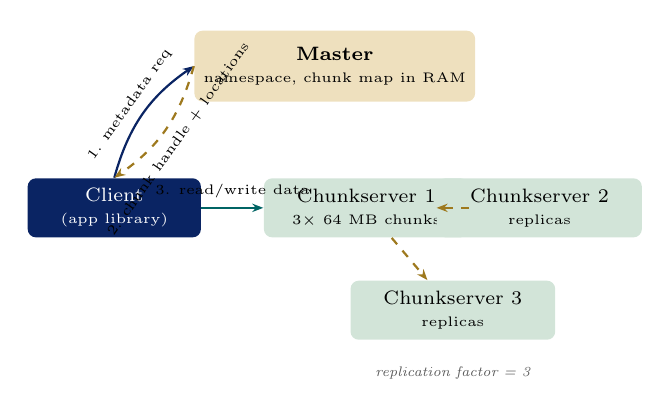
\begin{tikzpicture}[
          cbox/.style={rectangle, rounded corners=3pt, minimum width=2.6cm,
                       minimum height=0.75cm, align=center, font=\scriptsize},
          arr/.style={-{Stealth[length=4pt]}, draw=PUNavy, thick},
          darr/.style={-{Stealth[length=4pt]}, draw=PUGold!80!black, thick, dashed}
        ]
        % Master
        \node[cbox, fill=PUGold!30, minimum width=3.0cm, minimum height=0.9cm]
              (master) at (0, 3.6) {\textbf{Master}\\{\tiny namespace, chunk map in RAM}};

        % Client
        \node[cbox, fill=PUNavy, text=white, minimum width=2.2cm]
              (client) at (-2.8, 1.8) {Client\\{\tiny (app library)}};

        % Chunkservers
        \node[cbox, fill=PUGreen!20] (cs1) at (0.4, 1.8) {Chunkserver 1\\{\tiny 3$\times$ 64 MB chunks}};
        \node[cbox, fill=PUGreen!20] (cs2) at (2.6, 1.8) {Chunkserver 2\\{\tiny replicas}};
        \node[cbox, fill=PUGreen!20] (cs3) at (1.5, 0.5) {Chunkserver 3\\{\tiny replicas}};

        % Control path: client -> master
        \draw[arr]  (client.north) to[bend left=20]
              node[font=\tiny, above, sloped] {1. metadata req} (master.west);
        % Control path: master -> client
        \draw[darr] (master.west) to[bend left=20]
              node[font=\tiny, below, sloped] {2. chunk handle + locations}
              (client.north);
        % Data path: client -> chunkservers
        \draw[arr, draw=PUTeal] (client.east) --
              node[font=\tiny, above] {3. read/write data} (cs1.west);

        % Replication arrows
        \draw[darr] (cs1) -- (cs2);
        \draw[darr] (cs1) -- (cs3);
        \node[font=\tiny\itshape, text=PUGray] at (1.5, -0.3)
              {replication factor = 3};
      \end{tikzpicture}
      \end{center}
  \end{columns}
\end{frame}

%----------------------------------------------------------------
\begin{frame}{Technical Contribution 2 — Fault Tolerance \& Consistency}
  \begin{columns}[T]
    \column{0.50\textwidth}
      \begin{block}{Replication and Recovery}
        \begin{itemize}
          \item Every chunk replicated to \textbf{3 chunkservers} by default
          \item \textbf{Rack-aware placement}: primary replica on Rack~A,
                two secondaries on distinct Rack~B / C to survive rack-level
                power or switch failure
          \item Master heartbeats every chunkserver every \textbf{30 seconds};
                missing 3 heartbeats $\to$ re-replication begins automatically
          \item \textbf{Checksumming}: each 64~KB block within a chunk carries
                a 32-bit CRC; verified on every read — silent corruption caught
          \item \textbf{Stale replica detection}: chunk version numbers incremented
                on every lease grant; stale replicas are garbage collected
        \end{itemize}
      \end{block}

    \column{0.47\textwidth}
      \begin{block}{GFS Consistency Model}
        \renewcommand{\arraystretch}{1.3}
        \begin{tabular}{@{}lcc@{}}
          \toprule
          \textbf{Operation} & \textbf{Consistent?} & \textbf{Defined?} \\
          \midrule
          Serial write           & Yes & Yes \\
          Concurrent write       & Yes & No  \\
          Serial record append   & Yes & Yes \\
          Concurrent rec.\ append& No  & At records \\
          \bottomrule
        \end{tabular}
      \end{block}
      \vspace{5pt}
      \begin{exampleblock}{Atomic Record Append}
        Multiple clients append to the \emph{same} file concurrently.
        GFS guarantees each append is written \textbf{atomically at least once}
        at an offset chosen by the primary chunkserver.
        Readers may see padding or duplicates — handled by application-level
        sequence numbers (MapReduce uses this).
      \end{exampleblock}
  \end{columns}
\end{frame}

%----------------------------------------------------------------
\begin{frame}{Technical Contribution 3 — Master Design \& Leases}
  \begin{columns}[T]
    \column{0.52\textwidth}
      \begin{block}{Single-Master Metadata Management}
        \begin{itemize}
          \item All file namespace and chunk-location metadata kept
                \textbf{in master RAM}: $<$64 bytes per chunk $\times$
                millions of chunks = a few GB, affordable in 2003
          \item Namespace and chunk-ownership changes are logged to
                a \textbf{write-ahead operation log} on disk
                and replicated to \textbf{shadow master} replicas
          \item On master restart, the log is replayed;
                chunk locations are \textbf{not persisted} — chunkservers
                report their chunk inventory at startup (simpler, always fresh)
          \item Concern: single point of failure?\\
                Master restarts in \textbf{seconds} from log;
                shadow masters serve \emph{read-only} metadata during this window
        \end{itemize}
      \end{block}

    \column{0.45\textwidth}
      \begin{block}{Leases: Coordinating Concurrent Mutations}
        \begin{enumerate}
          \item Client requests write $\to$ asks master for chunk lease
          \item Master grants \textbf{60-second lease} to one
                ``primary'' chunkserver
          \item Primary defines a \textbf{serial mutation order};
                secondaries follow that order
          \item Data flows in a \textbf{pipeline}: client $\to$ nearest
                chunkserver $\to$ next $\to$ next (chain replication)
          \item Lease can be \textbf{extended} while writes are active;
                expires if master does not renew
        \end{enumerate}
      \end{block}
      \vspace{4pt}
      \begin{alertblock}{Separation of Control and Data}
        Control messages (lease grants, namespace ops) go through
        the master.
        Actual bytes \textbf{never touch the master} —
        a 1~Gbps master handles 1{,}000+ chunkservers at full throughput.
      \end{alertblock}
  \end{columns}
\end{frame}

%----------------------------------------------------------------
\begin{frame}{GFS vs.\ HDFS — Design Differences}
  \begin{center}
  \renewcommand{\arraystretch}{1.3}
  \begin{tabular}{@{}lll@{}}
    \toprule
    \textbf{Design Dimension} & \textbf{GFS (2003)} & \textbf{HDFS (2006+)} \\
    \midrule
    Language          & C++               & Java (JVM) \\
    Default chunk size& 64 MB             & 128 MB (configurable) \\
    Metadata store    & Master RAM + log  & NameNode RAM + edit log + FSImage \\
    HA for master     & Shadow masters    & Active/Standby NameNode (HDFS~2) \\
    Snapshots         & Supported (COW)   & Supported \\
    Random writes     & No (append-only)  & No \\
    Checksumming      & Per 64~KB block   & Per 512-byte chunk \\
    Replication       & 3 (rack-aware)    & 3 (rack-aware) \\
    Erasure coding    & No (GFS II / Colossus) & Yes (HDFS~3 EC) \\
    Open source       & No (proprietary)  & Yes (Apache License 2.0) \\
    \bottomrule
  \end{tabular}
  \end{center}
  \vspace{5pt}
  \begin{alertblock}{Key Lesson}
    HDFS is a \textbf{faithful open-source re-implementation} of GFS,
    not a derivative work — Ghemawat et al.\ published enough detail
    to reconstruct the system completely.
    The main deviations reflect ten years of production lessons
    and enterprise requirements (HA, erasure coding, federation).
  \end{alertblock}
\end{frame}

%----------------------------------------------------------------
\begin{frame}{Impact Today — Ghemawat et al.\ (2003)}
  \begin{columns}[T]
    \column{0.50\textwidth}
      \begin{block}{Direct Descendants}
        \begin{itemize}
          \item \textbf{HDFS} (2006) — the most deployed distributed
                filesystem in enterprise Big Data
          \item \textbf{Colossus} — Google's internal GFS successor
                (2010+); adds erasure coding, faster master
          \item \textbf{Amazon S3} (2006) — large-object storage shares
                the 64~MB+ block philosophy; immutable objects match
                GFS's append-only model
          \item \textbf{Azure Blob Storage / Google Cloud Storage} —
                same architectural lineage
          \item \textbf{Delta Lake / Apache Iceberg} (2019+) — write
                immutable Parquet files to object storage;
                the ``no random writes'' constraint is now a \emph{feature}
        \end{itemize}
      \end{block}

    \column{0.47\textwidth}
      \begin{exampleblock}{Stanford CS246 / MIT 6.830 Perspective}
        \begin{itemize}
          \item Stanford CS246 uses GFS as the canonical example of
                \textbf{system design under failure assumptions}:
                fault-tolerance via replication, not RAID
          \item MIT 6.830 covers the GFS consistency model as an
                instance of \textbf{relaxed consistency for throughput}:
                trading ``defined'' for ``consistent'' under concurrent appends
          \item CMU 15-721 frames GFS chunk servers as the earliest
                example of \textbf{shared-nothing distributed storage}
                for analytical workloads
        \end{itemize}
      \end{exampleblock}
      \vspace{4pt}
      \begin{alertblock}{CLO1 Connection}
        GFS directly instantiates the \textbf{Volume} and
        \textbf{Velocity} dimensions of Big Data (CLO1):
        petabyte-scale storage + high-throughput sequential I/O.
      \end{alertblock}
  \end{columns}
\end{frame}

%================================================================
\section{Case Study — Yahoo!\ Hadoop: 42{,}000 Nodes in Five Years}
%================================================================

%----------------------------------------------------------------
\begin{frame}{The Yahoo!\ Data Problem (2005)}
  \begin{columns}[T]
    \column{0.52\textwidth}
      \begin{block}{Why Yahoo!\ Needed a New Storage Layer}
        In 2005 Yahoo!\ operated:
        \begin{itemize}
          \item \textbf{Web crawler} (Nutch) producing 20+ TB/day of
                crawl data — unmanageable on a single-server NFS mount
          \item \textbf{Ad click logs}: 15 billion events per day
                requiring daily aggregation for billing
          \item \textbf{Email spam filter}: real-time classification
                over a corpus of 200M accounts
          \item \textbf{Personalisation}: user-activity logs for
                Yahoo!\ News, Finance, Sports — terabytes per property
          \item All of these ran on \emph{separate, siloed} infrastructure;
                sharing compute capacity was impossible
        \end{itemize}
      \end{block}

    \column{0.45\textwidth}
      \begin{alertblock}{The Turning Point}
        In January 2006, Yahoo!\ hired
        \textbf{Doug Cutting} — the creator of Apache Lucene and
        Nutch, who had already built an early HDFS prototype
        (then called NDFS) while reading the GFS and MapReduce papers.\\[5pt]
        Yahoo!\ gave Cutting a team and a mandate:
        \emph{build an open-source distributed computing platform
        that can run on Yahoo!'s existing commodity Linux clusters.}
      \end{alertblock}
      \vspace{5pt}
      \begin{exampleblock}{Project Name Origin}
        Doug Cutting named the project \textbf{Hadoop} after his
        son's toy yellow elephant — a name chosen because it was
        short, pronounceable, and had no prior meaning in computing.
      \end{exampleblock}
  \end{columns}
\end{frame}

%----------------------------------------------------------------
\begin{frame}{Yahoo!\ Hadoop Architecture (2008--2011)}
  \begin{columns}[T]
    \column{0.50\textwidth}
      \begin{block}{Cluster Growth Timeline}
        \renewcommand{\arraystretch}{1.25}
        \begin{tabular}{@{}rrl@{}}
          \toprule
          \textbf{Year} & \textbf{Nodes} & \textbf{Milestone} \\
          \midrule
          2007 & 1{,}000   & First production cluster \\
          2008 & 4{,}000   & 1~TB sort in 209 s (world record) \\
          2009 & 10{,}000  & Search index generation moved to Hadoop \\
          2010 & 26{,}000  & 100~PB stored; daily job count $>$10{,}000 \\
          2011 & 42{,}000  & Largest Hadoop cluster ever built at the time \\
          \bottomrule
        \end{tabular}
      \end{block}
      \vspace{5pt}
      \begin{exampleblock}{Hardware Specification (2008 commodity node)}
        \begin{itemize}\setlength\itemsep{0pt}
          \item 2$\times$ quad-core Intel Xeon @ 2.0 GHz
          \item 8 GB RAM
          \item 4$\times$ 1 TB SATA disks (no RAID)
          \item 1 Gbps Ethernet
          \item Rack: 40 nodes / 10 Gbps uplink
        \end{itemize}
      \end{exampleblock}

    \column{0.47\textwidth}
      \begin{center}
      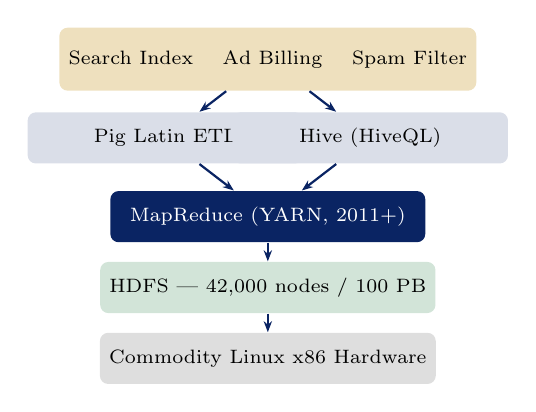
\begin{tikzpicture}[
          ybox/.style={rectangle, rounded corners=3pt, minimum width=3.5cm,
                       minimum height=0.65cm, align=center, font=\scriptsize},
          arr/.style={-{Stealth[length=4pt]}, draw=PUNavy, thick}
        ]
        \node[ybox, fill=PUGold!30, minimum height=0.8cm]
              (apps) at (0, 4.0)
              {Search Index \quad Ad Billing \quad Spam Filter};

        \node[ybox, fill=PUNavy!15] (pig)   at (-1.3, 3.0) {Pig Latin ETL};
        \node[ybox, fill=PUNavy!15] (hive)  at (1.3,  3.0) {Hive (HiveQL)};

        \node[ybox, fill=PUNavy, text=white, minimum width=4.0cm]
              (mr) at (0, 2.0) {MapReduce (YARN, 2011+)};

        \node[ybox, fill=PUGreen!20, minimum width=4.0cm]
              (hdfs) at (0, 1.1)
              {HDFS — 42{,}000 nodes / 100 PB};

        \node[ybox, fill=PUGray!20, minimum width=4.0cm]
              (hw) at (0, 0.2) {Commodity Linux x86 Hardware};

        \draw[arr] (apps)  -- (pig);
        \draw[arr] (apps)  -- (hive);
        \draw[arr] (pig)   -- (mr);
        \draw[arr] (hive)  -- (mr);
        \draw[arr] (mr)    -- (hdfs);
        \draw[arr] (hdfs)  -- (hw);
      \end{tikzpicture}
      \end{center}
  \end{columns}
\end{frame}

%----------------------------------------------------------------
\begin{frame}{Yahoo!'s Open-Source Contributions from Hadoop Operations}
  \begin{columns}[T]
    \column{0.52\textwidth}
      \begin{block}{What Yahoo!\ Built and Donated to Apache}
        Operating 42{,}000 nodes revealed gaps that Yahoo!\ engineers
        filled and then open-sourced:
        \begin{itemize}
          \item \textbf{Apache Pig} (2008) — dataflow language
                (Pig Latin) for ETL pipelines without Java MapReduce
          \item \textbf{Apache ZooKeeper} (2008) — distributed
                coordination service (named after the Hadoop zoo of projects);
                now used by Kafka, HBase, Pulsar
          \item \textbf{Apache Oozie} (2010) — workflow scheduler for
                DAGs of Hadoop jobs (replaced cron for multi-stage pipelines)
          \item \textbf{YARN} (2012, Hadoop 2.0) — resource manager
                that decoupled cluster resource management from MapReduce,
                enabling Spark, Tez, and others to run on the same cluster
          \item \textbf{HBase} co-development (2008) — modelled on
                Google Bigtable (Week 4 topic)
        \end{itemize}
      \end{block}

    \column{0.45\textwidth}
      \begin{alertblock}{Why Open Source Mattered}
        Yahoo!\ made a strategic bet: by open-sourcing Hadoop,
        they would \textbf{attract external developers} to fix bugs
        and add features without Yahoo!\ paying for the work.\\[5pt]
        This bet paid off:
        \begin{enumerate}
          \item Facebook, LinkedIn, Twitter adopted Hadoop
                — and contributed back Hive, Kafka, and Storm respectively
          \item Cloudera (2008) and Hortonworks (2011) formed as
                commercial Hadoop distributors
          \item 1{,}000+ contributors joined the Apache Hadoop project
                by 2013
        \end{enumerate}
      \end{alertblock}
      \vspace{5pt}
      \begin{exampleblock}{Benchmark: 2008 TeraSort Record}
        Yahoo!\ sorted \textbf{1 TB} of random data in
        \textbf{209 seconds} on a 910-node Hadoop cluster —
        a world record, using the GraySort benchmark.
      \end{exampleblock}
  \end{columns}
\end{frame}

%----------------------------------------------------------------
\begin{frame}{Lessons Learned \& Discussion Questions}
  \begin{columns}[T]
    \column{0.52\textwidth}
      \begin{block}{Key Lessons from the Yahoo!\ Case}
        \begin{enumerate}
          \item \textbf{Commodity hardware wins at scale}:
                42{,}000 low-cost nodes outperformed any single
                enterprise server at equivalent cost;
                failures became routine and manageable
          \item \textbf{GFS design scales to the real world}:
                HDFS implemented GFS faithfully and handled
                100~PB without fundamental redesign
          \item \textbf{Open source creates ecosystems}:
                Yahoo!'s Pig, ZooKeeper, and Oozie contributions
                seeded the entire modern data engineering toolchain
          \item \textbf{Workload shapes the API}:
                MapReduce's rigid two-phase model drove the
                need for Pig (higher-level) and later Spark
                (in-memory, multi-step DAGs)
          \item \textbf{Resource management is a first-class problem}:
                YARN's development shows that cluster scheduling
                becomes a bottleneck before storage does
        \end{enumerate}
      \end{block}

    \column{0.45\textwidth}
      \begin{alertblock}{Discussion Questions \textmd{\tiny (CLO1, CLO4)}}
        \begin{enumerate}
          \item GFS uses a \textbf{single master} holding all metadata
                in RAM.  Yahoo!\ eventually ran HDFS with a single
                NameNode on a 42{,}000-node cluster.
                Identify \textbf{two scalability bottlenecks} this
                creates and explain how HDFS~2 (YARN era) addressed them.
                \textit{[CLO1 — Understand]}
          \item Yahoo!'s 2008 TeraSort sorted 1~TB in 209~s on
                910 nodes, achieving $\approx$5~GB/s total throughput.
                If each node has a 1~Gbps NIC, calculate the
                \textbf{theoretical maximum network throughput} and
                explain why actual throughput was lower.
                \textit{[CLO4 — Analyse]}
          \item Yahoo!\ chose to \textbf{open-source Hadoop} rather
                than keep it proprietary.
                Discuss the strategic trade-offs and identify a
                counter-example where a company kept its distributed
                system proprietary.
                \textit{[CLO1 — Evaluate]}
        \end{enumerate}
      \end{alertblock}
  \end{columns}
\end{frame}

%================================================================
\section{Live Exercise}
%================================================================

%----------------------------------------------------------------
\begin{frame}[fragile]{Live Exercise — HDFS Block Simulation in Python}
  \begin{columns}[T]
    \column{0.50\textwidth}
      \begin{block}{Task (25 minutes, pairs)}
        Simulate the \textbf{GFS/HDFS block placement algorithm}
        without a real cluster.\\[5pt]
        \textbf{Goal}: given a 500~MB file and 64~MB blocks,
        distribute 3 replicas rack-aware across 6 nodes
        (2 racks, 3 nodes each). Print the block map.\\[5pt]
        \textbf{Rack-aware rule}:
        \begin{enumerate}\setlength\itemsep{1pt}
          \item Replica 1: random node on Rack A
          \item Replica 2: random \emph{different} node on Rack A
          \item Replica 3: random node on Rack B
        \end{enumerate}
        \textbf{Extension}: simulate a node failure and trigger
        re-replication to maintain factor = 3.
      \end{block}

    \column{0.47\textwidth}
      \begin{exampleblock}{Python Skeleton}
        \scriptsize
        \begin{verbatim}
import random, math

BLOCK_SIZE = 64  # MB
FILE_SIZE  = 500 # MB
REPL       = 3

racks = {
  "A": ["nodeA1","nodeA2","nodeA3"],
  "B": ["nodeB1","nodeB2","nodeB3"],
}

n_blocks = math.ceil(FILE_SIZE / BLOCK_SIZE)
block_map = {}

for b in range(n_blocks):
    r1 = random.choice(racks["A"])
    r2 = random.choice(
           [n for n in racks["A"] if n!=r1])
    r3 = random.choice(racks["B"])
    block_map[f"block_{b}"] = [r1, r2, r3]

for blk, nodes in block_map.items():
    print(f"{blk}: {nodes}")
        \end{verbatim}
      \end{exampleblock}
  \end{columns}
\end{frame}

%================================================================
\section*{References}
%================================================================

%----------------------------------------------------------------
\begin{frame}{References}
  \begin{block}{Seminal Paper}
    \begin{itemize}
      \item Ghemawat, S., Gobioff, H., \& Leung, S.-T. (2003).
            The Google File System.
            \textit{Proceedings of the 19th ACM SOSP}, 29--43.
    \end{itemize}
  \end{block}
  \vspace{4pt}
  \begin{block}{Textbooks \textmd{[TW], [SA], [TE]}}
    \begin{itemize}
      \item \textbf{[TW]} White, T. (2015).
            \textit{Hadoop: The Definitive Guide}, 4th ed.
            (Ch.~3 — HDFS; Ch.~2 — MapReduce Overview). O'Reilly.
      \item \textbf{[SA]} Acharya, S., \& Chellappan, S. (2015).
            \textit{Big Data and Analytics}
            (Ch.~3 — Hadoop Ecosystem). Wiley.
      \item \textbf{[TE]} Erl, T., Khattak, W., \& Buhler, P. (2016).
            \textit{Big Data Fundamentals}
            (Ch.~5 — Distributed Storage). Prentice Hall.
    \end{itemize}
  \end{block}
  \vspace{4pt}
  \begin{block}{Case Study Sources}
    \begin{itemize}
      \item Owen, S., Anil, R., Dunning, T., \& Friedman, E. (2011).
            \textit{Mahout in Action} (Yahoo!\ Hadoop case).
            Manning Publications.
      \item Borthakur, D. (2008).
            HDFS Architecture Guide. Apache Software Foundation.
    \end{itemize}
  \end{block}
\end{frame}

%----------------------------------------------------------------
\begin{frame}{Closing — Week 3, Part 2}
  \begin{columns}[T]
    \column{0.52\textwidth}
      \begin{block}{Key Takeaways}
        \begin{itemize}
          \item GFS (2003) proved that \textbf{commodity hardware + software
                fault-tolerance} outperforms expensive reliable hardware
                at web scale — the foundational insight of distributed storage
          \item \textbf{HDFS is GFS} re-implemented in Java;
                understanding GFS means understanding HDFS at depth
          \item Yahoo!'s 42{,}000-node cluster validated GFS design
                at industrial scale \emph{and} produced most of the
                tools (Pig, ZooKeeper, YARN, Oozie) we still use today
          \item The \textbf{append-only, large-block} design choice —
                made in 2003 for MapReduce — is still the dominant
                pattern in cloud object storage and Delta Lake today
        \end{itemize}
      \end{block}

    \column{0.45\textwidth}
      \begin{alertblock}{Quote of the Week}
        \begin{center}
        \large\itshape
        ``The system is designed for large\\
        streaming reads, not small random reads.\\
        Sustained bandwidth matters more\\
        than low latency.''
        \end{center}
        \begin{flushright}
        \small --- Ghemawat, Gobioff \& Leung (2003)
        \end{flushright}
      \end{alertblock}
      \vspace{6pt}
      \begin{exampleblock}{Part 1 Preview — Week 4}
        \textbf{MapReduce, Pig, Hive \& HBase}\\[3pt]
        \begin{itemize}\setlength\itemsep{1pt}
          \item MapReduce execution model and fault tolerance
          \item Pig Latin for ETL pipelines
          \item HiveQL and the metastore
          \item HBase as a Bigtable clone
        \end{itemize}
      \end{exampleblock}
  \end{columns}
\end{frame}

%=================================================================
\end{document}
%=================================================================
